\chapter{從開弦量子到快子與重力}

\lectureoverview{現在，我們將上一講求得的簡正模量子化，並探討它們會產生哪些粒子態。每個橫向模都是一個諧振子，但其歸一化方式稍微不同尋常：激發第\(n\)個模會使光前能量，因而也使質量平方能級，提高\(n\)個單位。開弦第一激發能級的變換性質，恰與無質量向量的兩種橫向極化相同。因此，相對論一致性要求基態的質量平方為負。這個態就是玻色弦快子；它真正代表的是不穩定的真空，而不是實際上可用的超光速粒子。最後，弦一旦發生交互作用，就會結合與分裂，因此閉弦無可避免；最低的閉弦激發態將是重力子。}

\section{藏在每個弦模中的諧振子}

對於一個橫向座標\(X\)，第\(n\)個非零簡正模的能量與拉格朗日量為

\begin{align}
  E_n
  &=
  \frac14\dot X_n^{\,2}
  +\frac{n^2}{4}X_n^2,
  \label{eq:l03-mode-energy}\\
  L_n
  &=
  \frac14\dot X_n^{\,2}
  -\frac{n^2}{4}X_n^2.
  \label{eq:l03-mode-lagrangian}
\end{align}

\(1/4\)的因子並非錯誤，而是記錄了將弦作用量化為彼此獨立的傅立葉模時所採用的歸一化方式。因此，建立哈密頓量的第一步是計算正則動量，

\begin{equation}
  p_n=\frac{\partial L_n}{\partial\dot X_n}
     =\frac12\dot X_n,
  \qquad
  \dot X_n=2p_n.
  \label{eq:l03-canonical-momentum}
\end{equation}

勒讓德變換得到

\begin{equation}
  H_n=p_n\dot X_n-L_n
     =p_n^2+\frac{n^2}{4}X_n^2.
  \label{eq:l03-mode-hamiltonian}
\end{equation}

\begin{figure}[H]
  \centering
  \includegraphics[width=0.82\textwidth]{lecture_03_figure_01.png}
  \caption{沿用開弦歸一化方式時，模的能量、拉格朗日量、正則動量與哈密頓量。}
  \lectureframe{00:05:40}
  \label{fig:l03-mode-hamiltonian-board}
\end{figure}

要將\(H_n\)因式分解，將\(X_n\)和\(p_n\)組合起來，得到

\begin{equation}
  \frac{nX_n}{2}\pm i p_n.
\end{equation}

在古典力學中，這兩個因子會彼此對易；但在量子力學中，

\begin{equation}
  [X_n,p_m]=i\delta_{nm}
  \label{eq:l03-canonical-commutator}
\end{equation}

在\(\hbar=1\)的單位制下。交叉項不會自行抵消。對於固定的模，

\begin{align}
  \left[\frac{nX_n}{2}+ip_n,
        \frac{nX_n}{2}-ip_n\right]
  &=n,
  \label{eq:l03-unscaled-commutator}\\
  \left(\frac{nX_n}{2}-ip_n\right)
  \left(\frac{nX_n}{2}+ip_n\right)
  &=H_n-\frac n2.
  \label{eq:l03-factorized-hamiltonian}
\end{align}

\begin{figure}[H]
  \centering
  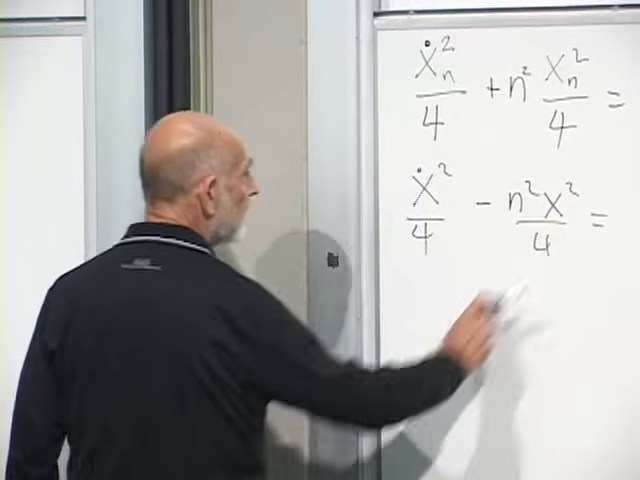
\includegraphics[width=0.82\textwidth]{lecture_03_figure_02.png}
  \caption{黑板上的計算顯示，正則對易關係帶來了\(n\)這個因子。}
  \lectureframe{00:10:30}
  \label{fig:l03-commutator-board}
\end{figure}

\(n\)這個因子告訴我們升降算符應如何歸一化：

\begin{align}
  a_n
  &\equiv
  \frac{\sqrt n}{2}X_n+\frac{i}{\sqrt n}p_n,
  \label{eq:l03-annihilator}\\
  a_n^\dagger
  &\equiv
  \frac{\sqrt n}{2}X_n-\frac{i}{\sqrt n}p_n.
  \label{eq:l03-creator}
\end{align}

它們滿足

\begin{equation}
  [a_n,a_m^\dagger]=\delta_{nm},
  \qquad
  H_n=n\left(a_n^\dagger a_n+\frac12\right).
  \label{eq:l03-oscillator-algebra}
\end{equation}

因此，\(a_n^\dagger\)會在第\(n\)個振子中增加一個量子，但該量子帶有\(n\)個單位的模能量。熟悉的諧振子能階間距並未消失；其頻率為\(\omega_n=n\)。

\begin{figure}[H]
  \centering
  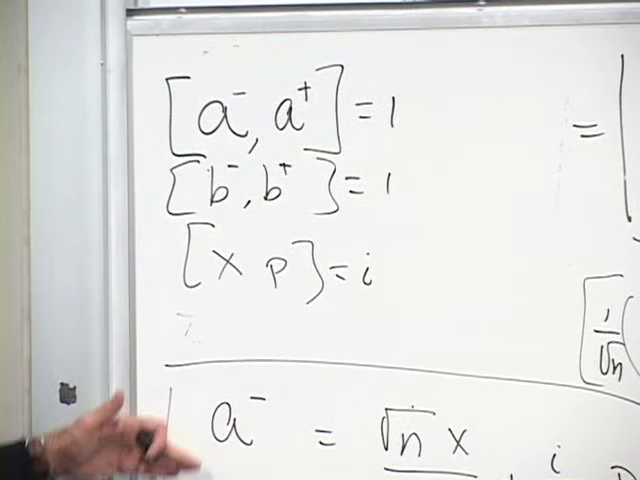
\includegraphics[width=0.82\textwidth]{lecture_03_figure_03.png}
  \caption{第\(n\)個弦振子的歸一化湮滅算符與產生算符。}
  \lectureframe{00:12:00}
  \label{fig:l03-ladder-board}
\end{figure}

\subsection{兩組橫向振子塔}

在四維時空中，沿\(z\)軸帶有極大動量的弦有兩個橫向座標\(X\)和\(Y\)。因此，我們需要兩組彼此獨立的振子塔。令\(a_n,a_n^\dagger\)作用於\(X\)模，\(b_n,b_n^\dagger\)作用於\(Y\)模。由\eqref{eq:l03-annihilator}--\eqref{eq:l03-creator}解出座標，可得

\begin{equation}
  X_n=\frac{a_n+a_n^\dagger}{\sqrt n},
  \qquad
  Y_n=\frac{b_n+b_n^\dagger}{\sqrt n}.
  \label{eq:l03-mode-coordinates}
\end{equation}

\begin{figure}[H]
  \centering
  \includegraphics[width=0.78\textwidth]{lecture_03_figure_04.png}
  \caption{以產生算符與湮滅算符表示模座標。}
  \lectureframe{00:17:05}
  \label{fig:l03-coordinate-operator-board}
\end{figure}

開弦座標以 Neumann 模展開：

\begin{align}
  X(\sigma,\tau)
  &=X_{\rm cm}(\tau)
    +\sum_{n=1}^{\infty}X_n(\tau)\cos(n\sigma),
  \label{eq:l03-X-fourier}\\
  Y(\sigma,\tau)
  &=Y_{\rm cm}(\tau)
    +\sum_{n=1}^{\infty}Y_n(\tau)\cos(n\sigma).
  \label{eq:l03-Y-fourier}
\end{align}

端點斜率為零，因此會出現餘弦。將\eqref{eq:l03-mode-coordinates}代入後，弦本身便成為算符：

\begin{align}
  X(\sigma,\tau)
  &=X_{\rm cm}(\tau)
    +\sum_{n=1}^{\infty}
      \frac{a_n(\tau)+a_n^\dagger(\tau)}{\sqrt n}
      \cos(n\sigma),
  \label{eq:l03-X-operator}\\
  Y(\sigma,\tau)
  &=Y_{\rm cm}(\tau)
    +\sum_{n=1}^{\infty}
      \frac{b_n(\tau)+b_n^\dagger(\tau)}{\sqrt n}
      \cos(n\sigma).
  \label{eq:l03-Y-operator}
\end{align}

\begin{figure}[H]
  \centering
  \begin{minipage}[t]{0.48\textwidth}
    \centering
    \includegraphics[width=\textwidth]{lecture_03_figure_05.png}
    \par\smallskip\footnotesize (a) 座標模展開。
  \end{minipage}\hfill
  \begin{minipage}[t]{0.48\textwidth}
    \centering
    \includegraphics[width=\textwidth]{lecture_03_figure_06.png}
    \par\smallskip\footnotesize (b) 將升降算符代入弦座標。
  \end{minipage}
  \caption{量子開弦的形狀由所有橫向振子算符共同構成。}
  \lectureframe{00:20:35 and 00:21:05}
  \label{fig:l03-string-coordinate-board}
\end{figure}

\begin{classroomqa}
\audiencequestion{\(X_n\)也是\(\sigma\)的函數嗎？\lecturetimestamp{00:21:48}}
\lecturerresponse{不是。對\(\sigma\)的依賴完全包含在\(\cos(n\sigma)\)中。係數\(X_n\)是該空間圖樣隨時間變化的振幅，因此\(X_n=X_n(\tau)\)。}
\end{classroomqa}

\begin{classroomqa}
\audiencequestion{為什麼稱為升算符和降算符的算符，看起來符號卻相反？\lecturetimestamp{00:23:13}}
\lecturerresponse{\(ip_n\)表面上的符號不是命名依據。計算它與哈密頓量的對易子即可判定。滿足\([H_n,a_n^\dagger]=n a_n^\dagger\)的算符會提高能量；滿足\([H_n,a_n]=-n a_n\)的算符則會降低能量。}
\end{classroomqa}

這兩組橫向振子塔是為了教學而採用的四維圖像。一致量子化的玻色弦具有二十六維時空，因此有二十四組橫向振子，而非兩組。以下的論證不變：第一能級態的數目必須與相同維度下無質量向量的物理極化數目相符。

\section{有質量粒子的自旋與無質量粒子的螺旋度}

在替弦態指定自旋之前，我們需要先明確區分兩者。有質量且自旋為\(J\)的粒子具有\(2J+1\)種自旋態，

\begin{equation}
  m_J=-J,-J+1,\ldots,J-1,J.
  \label{eq:l03-massive-spin-multiplet}
\end{equation}

例如，有質量的自旋一粒子有三種極化，有質量的自旋二粒子則有五種。我們可以轉到靜止系來理解原因。在靜止系中，所有空間旋轉都可進行。旋轉自旋軸，再變換回原來的參考系，所有\(2J+1\)個分量都屬於同一個相對論性粒子。

無質量粒子沒有靜止系。它的不變自旋標籤是螺旋度，也就是沿運動方向的角動量。光子只有\(h=+1\)和\(h=-1\)兩種螺旋度；重力子只有\(h=+2\)和\(h=-2\)兩種。純量有一個\(h=0\)態。本講以反射對稱性將兩種螺旋度配成一對。在手徵理論中，單一無質量不可約表示可能只帶有一種螺旋度，因此這種配對是額外的對稱性條件，並非僅由無質量這一性質所導致。\editorialnote{現代小群分類允許只有單一螺旋度的無質量表示。在熟悉的光子與重力子例子中，宇稱或適當補足 CPT 的場內容會提供相反的螺旋度。}

\begin{figure}[H]
  \centering
  \begin{minipage}[t]{0.45\textwidth}
    \centering
    \includegraphics[width=\textwidth]{lecture_03_figure_07.png}
    \par\smallskip\footnotesize (a) 黑板上開始進行的自旋態計數。
  \end{minipage}\hfill
  \begin{minipage}[t]{0.5\textwidth}
    \centering
    \begin{adjustbox}{max width=\linewidth}
    \begin{tabular}{@{}ccc@{}}
      \toprule
      自旋 & 有質量態 & 無質量螺旋度 \\
      \midrule
      \(0\) & \(1\) & \(0\) \\
      \(1\) & \(3\) & \(+1,-1\) \\
      \(2\) & \(5\) & \(+2,-2\) \\
      \bottomrule
    \end{tabular}
    \end{adjustbox}
  \end{minipage}
  \caption{有質量時，靜止系存在，也因此會有中間的自旋投影態。}
  \lectureframe{00:27:40}
  \label{fig:l03-spin-count}
\end{figure}

\subsection{光子的線偏振與圓偏振}

考慮一個沿\(z\)方向運動的光子。它的兩種橫向線偏振為\(\ket{x}\)和\(\ket{y}\)，但它們不是螺旋度本徵態。圓偏振態為

\begin{align}
  \ket{R}
  &=\frac{1}{\sqrt2}\left(\ket{x}+i\ket{y}\right),
  \label{eq:l03-right-circular}\\
  \ket{L}
  &=\frac{1}{\sqrt2}\left(\ket{x}-i\ket{y}\right),
  \label{eq:l03-left-circular}
\end{align}

其螺旋度分別為\(+1\)和\(-1\)；正負號取決於右旋與左旋的命名慣例。線偏振光子是這兩種結果的疊加。它的平均螺旋度可以為零，但螺旋度測量絕不會測得自旋為零的光子。同樣地，

\begin{equation}
  \frac{1}{\sqrt2}\left(\ket{x}+\ket{y}\right)
\end{equation}

只是偏振方向為四十五度的線偏振。

\begin{figure}[H]
  \centering
  \begin{minipage}[t]{0.48\textwidth}
    \centering
    \includegraphics[width=\textwidth]{lecture_03_figure_08.png}
    \par\smallskip\footnotesize (a) 黑板上的圓偏振態。
  \end{minipage}\hfill
  \begin{minipage}[t]{0.48\textwidth}
    \centering
    \begin{adjustbox}{max width=\linewidth}
    \begin{tikzpicture}[>=Latex,scale=0.9]
      \draw[->,thick] (0,0) -- (3.4,0) node[right] {\(z\)};
      \draw[->,blue!70!black,thick] (0,0) -- (0,2.0)
        node[above] {\(x\)};
      \draw[->,orange!85!black,thick] (0,0) -- (-1.4,-1.2)
        node[below left] {\(y\)};
      \draw[red!70!black,thick,->]
        plot[domain=0:320,samples=80]
        ({1.0*cos(\x)},{0.58*sin(\x)+0.4});
      \node[red!70!black] at (1.55,1.25) {circular};
    \end{tikzpicture}
    \end{adjustbox}
  \end{minipage}
  \caption{線偏振提供橫向基底；圓偏振組合則使螺旋度算符對角化。}
  \lectureframe{00:37:45}
  \label{fig:l03-polarization}
\end{figure}

\begin{classroomqa}
\audiencequestion{這和 Stern--Gerlach 實驗中的自旋態分離類似嗎？\lecturetimestamp{00:37:40}}
\lecturerresponse{量子疊加的概念相同，但描述光子時，直接使用的術語是偏振。圓偏振測量可以區分兩種螺旋度；光束中並沒有縱向、自旋為零的光子。}
\end{classroomqa}

自旋為二的重力子也呈現相同的模式。若只考慮自旋，可示意性地寫成

\begin{equation}
  \ket{+2}\sim\ket{+1}\otimes\ket{+1},
  \qquad
  \ket{-2}\sim\ket{-1}\otimes\ket{-1}.
  \label{eq:l03-graviton-helicity}
\end{equation}

這並不是說重力子真的是由兩個光子組成，而是說兩個相同的螺旋度相加後，會得到正確的自旋二螺旋度。

\begin{classroomqa}
\audiencequestion{雙光子的類比也適用於其他量子數嗎？\lecturetimestamp{00:41:05}}
\lecturerresponse{不能把它當作組成模型。有些重要公式會將重力振幅表示為規範理論振幅的乘積，或``平方，''但重力子仍是獨立的粒子。此處最可靠的類比，是把它視為螺旋度的陳述。\editorialnote{現代的 Kawai--Lewellen--Tye 關係與雙重拷貝關係，能在適當的理論中精確描述振幅間的關係；但它們並不會把重力子變成兩個光子的束縛態。}}
\end{classroomqa}

\begin{classroomqa}
\audiencequestion{光子可以有任意動量，因此它的譜不是連續的嗎？粒子所要求的不是孤立的譜嗎？\lecturetimestamp{00:42:17}}
\lecturerresponse{連續變數是質心動量。固定這個動量，再檢視內部的不變質量。粒子由孤立的質量能級來識別；改變粒子的整體動量，則會得到通常的連續色散關係。}
\end{classroomqa}

\section{最低的開弦能級}

現在可以回到弦。在大動量描述中，有限的內部光前能量與不變質量平方成正比。暫略整體的弦尺度，將譜寫成

\begin{equation}
  \begin{aligned}
    M^2
    &=m_0^2
      +\sum_{n=1}^{\infty}n
       \left(N_n^{(a)}+N_n^{(b)}\right),\\
    N_n^{(a)}&=a_n^\dagger a_n,
    \qquad
    N_n^{(b)}=b_n^\dagger b_n.
  \end{aligned}
  \label{eq:l03-open-spectrum}
\end{equation}

振子基態滿足

\begin{equation}
  a_n\ket{0}=0,
  \qquad
  b_n\ket{0}=0,
  \qquad n=1,2,\ldots .
  \label{eq:l03-ground-annihilation}
\end{equation}

這不是弦不存在，而是量子弦的最低激發態；它的座標仍會漲落。令其質量平方為\(m_0^2\)，目前尚未決定。

\begin{figure}[H]
  \centering
  \includegraphics[width=0.78\textwidth]{lecture_03_figure_09.png}
  \caption{開弦基態，以及定義此基態的湮滅條件。}
  \lectureframe{00:45:20}
  \label{fig:l03-ground-state-board}
\end{figure}

能量最低的激發使用\(n=1\)產生算符：

\begin{equation}
  a_1^\dagger\ket{0},
  \qquad
  b_1^\dagger\ket{0},
  \qquad
  M^2=m_0^2+1.
  \label{eq:l03-first-level}
\end{equation}

\begin{figure}[H]
  \centering
  \includegraphics[width=0.78\textwidth]{lecture_03_figure_10.png}
  \caption{兩個簡併的第一能級態之一；黑板上也寫出了它的質量平方增量。}
  \lectureframe{00:49:25}
  \label{fig:l03-first-level-board}
\end{figure}

「``一''」在式{eq:l03-first-level}中並非一焦耳、一電子伏特或一普朗克質量。我們省略了有量綱的弦尺度。目前它表示振子的質量平方階梯上的一個步階；缺少的單位將在下一堂課補回。

這兩個簡併態的任意線性組合也都是此能級上的態。特別是，

\begin{equation}
  \frac{1}{\sqrt2}
  \left(a_1^\dagger\pm i b_1^\dagger\right)\ket{0}
  \label{eq:l03-string-circular-states}
\end{equation}

這是弦的圓偏振類比。在\(x\)-\(y\)平面內旋轉時，\(a_1^\dagger\)和\(b_1^\dagger\)的變換方式如同橫向向量的兩個分量。因此，\eqref{eq:l03-string-circular-states}中的組合具有螺旋度\(+1\)和\(-1\)。

\begin{figure}[H]
  \centering
  \includegraphics[width=0.82\textwidth]{lecture_03_figure_11.png}
  \caption{黑板上整理了基態條件、兩個第一能級激發態，以及它們的圓偏振組合。}
  \lectureframe{00:56:00}
  \label{fig:l03-level-structure-board}
\end{figure}

沒有第三個簡併態可作為縱向極化。如果這兩個態有非零質量，則自旋一的相對論性粒子需要三種極化。但這裡恰好只有兩種，因此此態必須是無質量的。於是

\begin{equation}
  m_0^2+1=0,
  \qquad
  m_0^2=-1.
  \label{eq:l03-intercept-condition}
\end{equation}

第一能級具有光子般的性質：它是無質量的規範向量態，但不一定是電磁學中的光子；它最終對應哪種規範場，取決於弦模型。其下方的基態具有負質量平方，這就是玻色開弦的快子。\editorialnote{在完整的臨界玻色弦中，正規序截距與洛侖茲代數都和\(D=26\)有關。本講只考慮兩個橫向方向，是同一套態計數論證在四維中的呈現：\(D-2\)個第一能級振子態，恰與無質量向量的\(D-2\)個物理極化相符。}

\begin{classroomqa}
\audiencequestion{為什麼我們需要在意\(m_0^2\)是負的？\lecturetimestamp{00:56:35}}
\lecturerresponse{因為質量平方代表二次場勢在我們稱為真空的態附近的曲率。曲率為負，表示這個構型不是穩定的基態。接下來的計算會將此說法表達得更精確。}
\end{classroomqa}

\section{快子的真正意義}

``快子''這個名稱容易讓人一開始就產生誤解。先從\(c=1\)的相對論色散關係出發，

\begin{equation}
  E(p)=\sqrt{p^2+m^2}.
  \label{eq:l03-relativistic-dispersion}
\end{equation}

對於波包，群速度為

\begin{equation}
  v_g=\frac{dE}{dp}.
  \label{eq:l03-group-velocity}
\end{equation}

這會得到熟悉的情形：

\begin{align}
  E_{\rm nr}(p)&=\frac{p^2}{2m},
  &v_g&=\frac{p}{m},
  \label{eq:l03-nr-group-velocity}\\
  E_\gamma(p)&=|p|,
  &|v_g|&=1,
  \label{eq:l03-photon-group-velocity}\\
  E_m(p)&=\sqrt{p^2+m^2},
  &|v_g|&=\frac{|p|}{\sqrt{p^2+m^2}}<1.
  \label{eq:l03-massive-group-velocity}
\end{align}

\begin{figure}[H]
  \centering
  \begin{minipage}[t]{0.48\textwidth}
    \centering
    \includegraphics[width=\textwidth]{lecture_03_figure_12.png}
    \par\smallskip\footnotesize (a) 非相對論性的群速度。
  \end{minipage}\hfill
  \begin{minipage}[t]{0.48\textwidth}
    \centering
    \includegraphics[width=\textwidth]{lecture_03_figure_13.png}
    \par\smallskip\footnotesize (b) 相對論性色散關係及其導數。
  \end{minipage}
  \caption{由\(E(p)\)的斜率讀出傳播速度。}
  \lectureframe{01:01:50 and 01:03:15}
  \label{fig:l03-group-velocity-board}
\end{figure}

若\(m^2=-\mu^2\)，形式上便得到

\begin{equation}
  E(p)=\sqrt{p^2-\mu^2},
  \qquad
  v_g=\frac{p}{\sqrt{p^2-\mu^2}},
  \label{eq:l03-formal-tachyon-dispersion}
\end{equation}

只要平方根內的量為實數，就有\(|v_g|>1\)。但這並非玻色弦基態的正確物理解釋。低動量時頻率已是虛數，問題在此便已顯現。

\subsection{場勢的負曲率}

考慮一維空間中的實純量場，

\begin{equation}
  \left(\partial_t^2-\partial_x^2+m^2\right)\phi=0.
  \label{eq:l03-klein-gordon}
\end{equation}

對於平面波\(\phi\propto e^{-i\omega t+ikx}\)，

\begin{equation}
  \omega^2=k^2+m^2.
  \label{eq:l03-kg-dispersion}
\end{equation}

\begin{figure}[H]
  \centering
  \includegraphics[width=0.82\textwidth]{lecture_03_figure_14.png}
  \caption{用來揭示負質量平方所導致不穩定性的 Klein--Gordon 方程。}
  \lectureframe{01:06:40}
  \label{fig:l03-klein-gordon-board}
\end{figure}

守恆的二次能量為

\begin{equation}
  \mathcal E
  =\frac12\int dx\,
  \left[
    \dot\phi^{\,2}
    +(\partial_x\phi)^2
    +m^2\phi^2
  \right].
  \label{eq:l03-field-energy}
\end{equation}

\begin{figure}[H]
  \centering
  \includegraphics[width=0.82\textwidth]{lecture_03_figure_15.png}
  \caption{純量場的能量，其中質量項決定勢能在局部的曲率。}
  \lectureframe{01:08:10}
  \label{fig:l03-field-energy-board}
\end{figure}

當\(m^2>0\)時，局部勢能\(V(\phi)=\tfrac12m^2\phi^2\)呈碗狀，構型\(\phi=0\)位於碗底。若\(m^2=-\mu^2\)，同一點便是倒置碗狀勢能的頂端。方程\eqref{eq:l03-kg-dispersion}變為

\begin{equation}
  \omega^2=k^2-\mu^2.
  \label{eq:l03-tachyonic-modes}
\end{equation}

對於\(k^2<\mu^2\)的模，

\begin{equation}
  \omega=\pm i\sqrt{\mu^2-k^2},
  \qquad
  \phi_k(t)\propto
  e^{\pm\sqrt{\mu^2-k^2}\,t}.
  \label{eq:l03-growing-mode}
\end{equation}

其中一個分支會指數增長。因此，所謂的真空並不穩定：任意微小的長波長擾動都會使場偏離\(\phi=0\)。這就是譜中出現快子的意義。

\subsection{倒立擺鏈}

一排彼此耦合的擺能清楚呈現這個差異。讓每個擺都保持直立。這個均勻構型確實存在，但它在勢能極大值處達到平衡。只要輕推其中一個擺，它就會倒下並牽動鄰近的擺。倒下的前沿會以耦合所決定的有限訊號速度沿著鏈傳播。

\begin{figure}[H]
  \centering
  \begin{minipage}[t]{0.48\textwidth}
    \centering
    \includegraphics[width=\textwidth]{lecture_03_figure_16.png}
    \par\smallskip\footnotesize (a) 黑板上的耦合直立擺模型。
  \end{minipage}\hfill
  \begin{minipage}[t]{0.48\textwidth}
    \centering
    \begin{adjustbox}{max width=\linewidth}
    \begin{tikzpicture}[>=Latex,scale=0.78]
      \draw[thick] (-0.3,0) -- (6.3,0);
      \foreach \x/\a in {0/0,1/0,2/8,3/28,4/55,5/72,6/78}{
        \fill (\x,0) circle (0.06);
        \draw[thick] (\x,0) -- ++({90-\a}:1.25);
        \fill[blue!65!black]
          ($(\x,0)+({90-\a}:1.25)$) circle (0.11);
      }
      \draw[red!70!black,->,thick] (1.7,-0.45) -- (4.6,-0.45)
        node[midway,below] {falling front};
    \end{tikzpicture}
    \end{adjustbox}
  \end{minipage}
  \caption{即使系統的線性化譜包含負質量平方，不穩定性仍會以符合因果律的方式傳播。}
  \lectureframe{01:10:40}
  \label{fig:l03-pendulum-instability}
\end{figure}

這個機制不允許任何受控訊號超越因果前沿。快子模指出的是錯誤的展開點，而不是穩定的超光速訊息載體。\editorialnote{對於局域相對論性場方程，前沿速度仍是因果速度。實數的高\(k\)分支所具有的形式群速度，並不會讓不穩定真空成為超光速通訊通道。}

\begin{classroomqa}
\audiencequestion{剛才找到的無質量態，就是弦理論所預言的重力子嗎？\lecturetimestamp{01:14:27}}
\lecturerresponse{不是。它是開弦的自旋一態，具有兩種極化，因此類似規範玻色子。重力子則是閉弦的自旋二激發態。}
\end{classroomqa}

\begin{classroomqa}
\audiencequestion{倒置的勢在數學上可以成立嗎？系統倒下後會停在哪裡？\lecturetimestamp{01:15:17}}
\lecturerresponse{這完全可以作為局部近似，但單靠這個近似並沒有基態，因為能量沒有下界。更完整的勢能可能會再次向上彎曲，並具有更低的極小值。接著，系統會朝那個穩定構型滾落或凝聚。}
\end{classroomqa}

普通玻色弦正有這個缺陷。較高的振子態仍屬於譜的一部分，但它們是建立在不穩定背景上的激發態。一致的超弦理論會在穩定扇區中排除開弦快子，同時保留無質量與有質量的弦激發態。

\begin{classroomqa}
\audiencequestion{除了兩種極化之外，這個開弦態的其他性質也和光子相符嗎？\lecturetimestamp{01:17:07}}
\lecturerresponse{這個態的行為如同無質量規範玻色子。它具體的電荷指派、輻射規則與粒子身分都取決於弦模型，因此應稱它為類光子態，而不宜立刻認定它就是電磁作用中的光子。這些交互作用性質會在後續討論。}
\end{classroomqa}

\section{弦的交互作用}

自由弦的譜只涵蓋理論的一半，弦也會結合與分裂。首先可以先記住，激發態的自由弦能帶有角動量。一根筆直的旋轉弦會繞著質心轉動，其能量與角動量會沿著熟知的弦狀軌跡一同增加。

\begin{figure}[H]
  \centering
  \includegraphics[width=0.72\textwidth]{lecture_03_figure_17.png}
  \caption{以質心為中心旋轉的開弦示意圖。}
  \lectureframe{01:19:30}
  \label{fig:l03-rotating-string-board}
\end{figure}

\begin{classroomqa}
\audiencequestion{自由弦能以一個固定端點為軸，端對端地旋轉嗎？\lecturetimestamp{01:20:02}}
\lecturerresponse{沒有錨定物就不行。自由的孤立系統會繞質心旋轉。如果一個端點連接到另一個物體或膜上，整個系統便能繞不同的中心旋轉；就像電子和原子核繞著共同質心運行，但質量大得多的原子核看起來幾乎固定不動。}
\end{classroomqa}

\subsection{開弦頂點}

對開弦而言，基本交互作用發生於兩個端點在同一時空點相遇之時。兩端點結合成一條弦的振幅為\(g_s\)。反向演化則對應一條弦分裂成兩條弦的振幅。示意如下：

\begin{equation}
  \text{open}+\text{open}
  \quad\rightleftarrows\quad
  \text{open}.
  \label{eq:l03-open-joining}
\end{equation}

\begin{figure}[H]
  \centering
  \begin{minipage}[t]{0.48\textwidth}
    \centering
    \includegraphics[width=\textwidth]{lecture_03_figure_18.png}
    \par\smallskip\footnotesize 黑板上的結合過程。
  \end{minipage}\hfill
  \begin{minipage}[t]{0.48\textwidth}
    \centering
    \begin{tikzpicture}[>=Latex,scale=0.9]
      \draw[->] (0,-2.1) -- (0,2.2) node[above] {time};
      \draw[blue!70!black,thick] (-2,-1.6) .. controls (-1.3,-0.9)
        and (-0.7,-0.35) .. (0,0);
      \draw[blue!70!black,thick] (2,-1.6) .. controls (1.3,-0.9)
        and (0.7,-0.35) .. (0,0);
      \draw[orange!85!black,thick] (0,0) .. controls (0.25,0.7)
        and (-0.15,1.25) .. (0.15,1.9);
      \fill[red!70!black] (0,0) circle (0.09);
      \node[right] at (0.12,0) {\(g_s\)};
    \end{tikzpicture}
  \end{minipage}
  \caption{端點結合是弦的局域粒子交互作用頂點；時間反演則對應分裂。}
  \lectureframe{01:24:05}
  \label{fig:l03-open-vertex}
\end{figure}

耦合是振幅。對於某個指定的基本過程，其相應機率的最低階項為\(|g_s|^2\)；相空間與歸一化因子則由完整計算給出。因此，將\(g_s\)稱為``機率''只是一種非正式的簡稱；區分振幅與機率，才能避免錯誤地多取一次平方。

交互作用的形式不取決於外部弦當下是在振動、旋轉，或處於其他振子態。這些態會改變矩陣元的細節，但採用的仍是同一種局域結合規則。

\subsection{開弦可以自行閉合}

假設一條開弦的兩個端點相遇。結合規則無法辨別它們是否屬於同一條弦，因此兩端點可以融合，形成一個閉合環：

\begin{equation}
  \text{open}\longrightarrow\text{closed}.
  \label{eq:l03-self-closing}
\end{equation}

\begin{figure}[H]
  \centering
  \begin{minipage}[t]{0.48\textwidth}
    \centering
    \includegraphics[width=\textwidth]{lecture_03_figure_19.png}
    \par\smallskip\footnotesize (a) 開弦讓兩個端點彼此靠近。
  \end{minipage}\hfill
  \begin{minipage}[t]{0.48\textwidth}
    \centering
    \begin{tikzpicture}[>=Latex,scale=0.92]
      \draw[blue!70!black,thick]
        (-2,0) .. controls (-1.2,1.5) and (1.2,1.5) .. (2,0);
      \fill[red!70!black] (-2,0) circle (0.08);
      \fill[red!70!black] (2,0) circle (0.08);
      \draw[->,thick] (-0.45,-0.45) -- (0.45,-0.45);
      \draw[orange!85!black,thick] (0,-1.55) ellipse (1.15 and 0.58);
      \node at (0,-2.25) {closed string};
    \end{tikzpicture}
  \end{minipage}
  \caption{有交互作用的開弦必然會產生閉弦。}
  \lectureframe{01:27:20}
  \label{fig:l03-open-becomes-closed}
\end{figure}

這並非可有可無的額外內容。任何包含開弦交互作用的理論都必須包含閉弦態。反向過程則允許閉弦在具備適當的端點與邊界條件時轉變為開弦。

\begin{classroomqa}
\audiencequestion{弦融合或分裂時，它們的振子能量會改變嗎？理論會決定能量如何改變嗎？\lecturetimestamp{01:28:05}}
\lecturerresponse{會。整個過程的能量與動量都守恆，而激發能則可以在出射弦之間重新分配。躍遷振幅由交互作用頂點與外部波函數決定。}
\end{classroomqa}

\subsection{閉弦之間的交互作用不必產生開弦}

這種推論只適用於單一方向：有交互作用的開弦需要閉弦，但理論可以只從閉弦開始。兩個閉合環可以接觸、重新連接，並合併成一個閉合環；反向過程則會使一個環分裂成兩個。整個過程不需要出現開弦端點。

\begin{figure}[H]
  \centering
  \begin{minipage}[t]{0.48\textwidth}
    \centering
    \includegraphics[width=\textwidth]{lecture_03_figure_20.png}
    \par\smallskip\footnotesize 黑板上的閉弦融合過程。
  \end{minipage}\hfill
  \begin{minipage}[t]{0.48\textwidth}
    \centering
    \begin{tikzpicture}[>=Latex,scale=0.88]
      \draw[blue!70!black,thick] (-1.35,0) circle (0.75);
      \draw[blue!70!black,thick] (1.35,0) circle (0.75);
      \draw[->,thick] (-0.35,-1.15) -- (0.35,-1.15);
      \draw[orange!85!black,thick] (0,-2.3) ellipse (1.35 and 0.68);
      \node at (0,1.2) {closed \(+\) closed};
      \node at (0,-3.25) {closed};
    \end{tikzpicture}
  \end{minipage}
  \caption{閉弦有自己的結合與分裂交互作用，不必經過開弦態。}
  \lectureframe{01:29:05}
  \label{fig:l03-closed-fusion}
\end{figure}

\begin{classroomqa}
\audiencequestion{若理論以閉弦為起點，也必須包含開弦嗎？\lecturetimestamp{01:28:35}}
\lecturerresponse{不必。閉弦可以透過重新連接彼此交互作用，並在整個過程中保持閉合。開弦則需要額外的邊界資料，例如允許的端點或膜。}
\end{classroomqa}

\section{為什麼引力無可避免}

閉弦振子的計算與開弦相似，但閉弦具有彼此獨立的左行與右行激發。兩者最低的非平凡匹配能級中包含無質量的自旋二態，其螺旋度正是重力子的螺旋度。因此，每個一致的閉弦交互作用理論都包含引力。

\begin{classroomqa}
\audiencequestion{為什麼最低的閉弦激發態必定是重力子，就像開弦能級必定是類光子態一樣？
\lecturetimestamp{01:30:59}}
\lecturerresponse{答案是同一類型的態計數，不過現在考慮的是左行與右行振子向量。它們的張量積包含無質量、對稱且無跡的自旋二極化態。下一講會詳細推導閉弦的譜；目前的重點是這個態的存在無可避免。}
\end{classroomqa}

開弦與閉弦也能彼此交互作用。閉環可以與開弦相遇並被吸收，使開弦變得更長，或轉變成不同的激發態。反過來，開弦也可以放射出閉環。在粒子層次上，這代表物質發射或吸收重力子。

\begin{figure}[H]
  \centering
  \begin{minipage}[t]{0.48\textwidth}
    \centering
    \includegraphics[width=\textwidth]{lecture_03_figure_21.png}
    \par\smallskip\footnotesize 弦段的局域重新連接。
  \end{minipage}\hfill
  \begin{minipage}[t]{0.48\textwidth}
    \centering
    \includegraphics[width=\textwidth]{lecture_03_figure_22.png}
    \par\smallskip\footnotesize 閉環連接到開弦上。
  \end{minipage}
  \caption{混合開--閉弦交互作用的黑板圖示，以及重力子交換普遍可能存在的原因。}
  \lectureframe{01:33:10 and 01:34:35}
  \label{fig:l03-mixed-interactions-board}
\end{figure}

\begin{figure}[H]
  \centering
  \begin{tikzpicture}[>=Latex,scale=0.88]
    \draw[blue!70!black,thick]
      (-3,-0.5) .. controls (-1.7,-0.1) and (-0.8,0.2) .. (0,0);
    \draw[blue!70!black,thick]
      (0,0) .. controls (0.9,0.3) and (2.0,0.1) .. (3,0.55);
    \draw[orange!85!black,thick] (-0.8,1.55) ellipse (0.75 and 0.45);
    \draw[->,red!70!black,thick] (-0.45,1.15) -- (-0.05,0.35);
    \node[blue!70!black] at (-2.2,-0.95) {open string};
    \node[orange!85!black] at (-0.8,2.25) {closed string};
    \node at (1.75,-0.5) {excited open string};
  \end{tikzpicture}
  \caption{不含時空背景的閉弦被開弦吸收之示意圖。}
  \label{fig:l03-mixed-interaction-redraw}
\end{figure}

每種弦態都能與重力子耦合，因為每條弦都帶有能量與動量，而且結合規則允許閉弦交換。這就是弦理論中引力具有普適性的由來。

\begin{classroomqa}
\audiencequestion{閉弦能轉變成開弦嗎？或者，它能在不違反端點規則的情況下與開弦結合嗎？\lecturetimestamp{01:31:20}}
\lecturerresponse{若理論同時包含這兩種扇區，閉弦可以附著到開弦上並改變開弦的狀態。單獨一條閉弦能否直接轉變成開弦，則取決於理論是否提供了合乎條件的端點。局域重新連接規則仍然相同。}
\end{classroomqa}

\begin{classroomqa}
\audiencequestion{閉合弦圈能否永久地彼此連結或打結？\lecturetimestamp{01:35:10}}
\lecturerresponse{在弱耦合下，弦大多近乎透明：除非微小的重聯振幅發揮作用，否則它們可以彼此穿過。因此，連結或結可以維持一段時間，但在允許的弦相互作用發生時，拓撲便可能改變。}
\end{classroomqa}

\begin{classroomqa}
\audiencequestion{相互作用機率是否與弦的狀態或速度無關？\lecturetimestamp{01:36:09}}
\lecturerresponse{局域耦合是同一個參數，但總躍遷機率也取決於波函數，以及相關部分彼此接觸的時間長短。快速相遇通常比緩慢相遇提供較短的相互作用時間。}
\end{classroomqa}

\section{仍未補上的尺度與耦合}

有兩項量綱上的處理刻意先擱置。第一，\(X\) 是長度，而 \(a_n\) 是無量綱的，因此 \eqref{eq:l03-mode-coordinates} 中的比例關係必須包含一個長度尺度。第二，振子能級提高時，不可能真的把一個無量綱數加到物理質量平方上。補回弦長 \(\ell_s\)，或等價地補回 Regge 斜率 \(\alpha'\sim\ell_s^2\)，就能補上缺少的量綱：

\begin{equation}
  M^2\sim\frac{1}{\alpha'}(N-a).
  \label{eq:l03-dimensional-spectrum}
\end{equation}

精確的約定與正規化將在下一講中確定。

\begin{classroomqa}
\audiencequestion{弦長的尺度，以及一個產生算符所增加的質量，由什麼決定？\lecturetimestamp{01:37:03}}
\lecturerresponse{有一個帶量綱的常數被省略了。它就是弦尺度，通常寫作 \(\ell_s\) 或 \(\alpha'\)。振子算符是無量綱的；弦尺度的冪次會將振子的能級數轉換為物理長度、張力與質量平方。}
\end{classroomqa}

第二個參數是弦耦合 \(g_s\)。在最簡單的討論中，它是一個控制弦的結合與分裂的普適數值。在較豐富的模型中，端點可以帶有不同標記，弦也可以在交會處相接。Y 形構型是三條通量管相遇的弦論類比；在早期的強子圖像中，它與三夸克重子相關，而一段單獨的開弦則類似夸克--反夸克介子。

\begin{classroomqa}
\audiencequestion{不同的弦端點能否有不同的結合機率？\lecturetimestamp{01:39:31}}
\lecturerresponse{最簡單的模型採用單一耦合。更精細的理論會在端點上附加荷或邊界標記，再由選擇定則決定哪些結合過程允許發生。詳細構造留待之後討論，但普適的局域結合概念仍然成立。}
\end{classroomqa}

\begin{classroomqa}
\audiencequestion{弦能否沿長度方向分裂，或形成 Y 形交會？\lecturetimestamp{01:40:01}}
\lecturerresponse{某些弦系統確實允許交會。這不是剛才所畫的普通雙端點分裂過程；只有當理論具有相容的弦荷時，才會出現這類交會。介子--重子通量管的類比有助於理解兩者的區別。}
\end{classroomqa}

\begin{classroomqa}
\audiencequestion{改變時空維度會改變相互作用耦合嗎？\lecturetimestamp{01:42:25}}
\lecturerresponse{維度會改變譜、相空間，以及緊緻化後得到的有效耦合。基本弦耦合仍然決定微擾展開的組織方式，但它在低維理論中的表現取決於額外維度的幾何與體積。}
\end{classroomqa}

\begin{classroomqa}
\audiencequestion{自由弦一開始運動，是由引力造成的嗎？\lecturetimestamp{01:43:17}}
\lecturerresponse{維持運動不需要力。初始位置與速度決定一個自由解；慣性使弦持續運動。引力或其他力會改變它的運動。追問初始條件由何而來，是另一個問題，不屬於局域運動方程的一部分。}
\end{classroomqa}

因此，我們得到三個彼此相關的結論。將開弦量子化，會在第一激發能級得到一個無質量向量；位於其下的玻色弦基態是不穩定的；而弦的相互作用必然會引入閉弦，其譜中包含引力。接下來要補回缺少的尺度，並明確地進行閉弦量子化。